\section{Implementation}
\subsection{Customizer}

\begin{figure}[H] 
	\centering 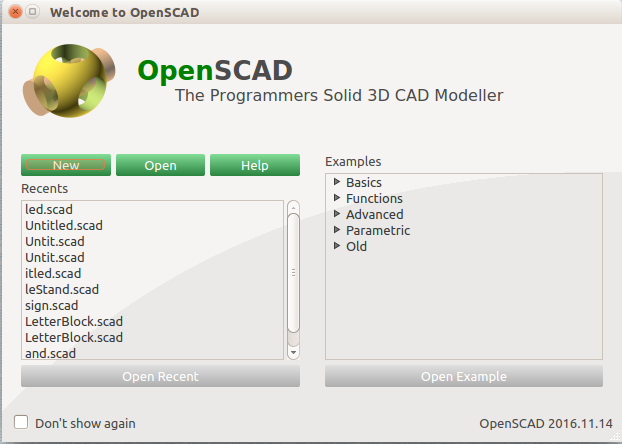
\includegraphics[scale=0.40]{images/output/1.png}
	\caption{StartUp Screen for OpenSCAD}
	\label{fig:1}
\end{figure}

Customizer  will provide User Interface to Customize Models interactively instead of modifying them manually. It will make the user able to create the templates for given model which can further be customize to cater to their need of different users and also provide feature to save the set of parameters which define a different model using same template of model.
\subsection{Activation of Customizer functions}
\begin{itemize}
	
	\item This is experimental functionality.So, Initially 
	OpenSCAD will look like \ref{fig:Normal OpenSCAD}
	\item In [Edit] menu, select [Preferences] then open tab [Features], tick Customizer, then close the window when tick shown \ref{fig:3}.
    \item In View menu, you shall now have an option [Hide customizer], that you shall untick. Then you will be able to see the customizer \ref{fig:OpenSCAD with Customizer}
    
\end{itemize}

\begin{figure}[H] 
   	\centering 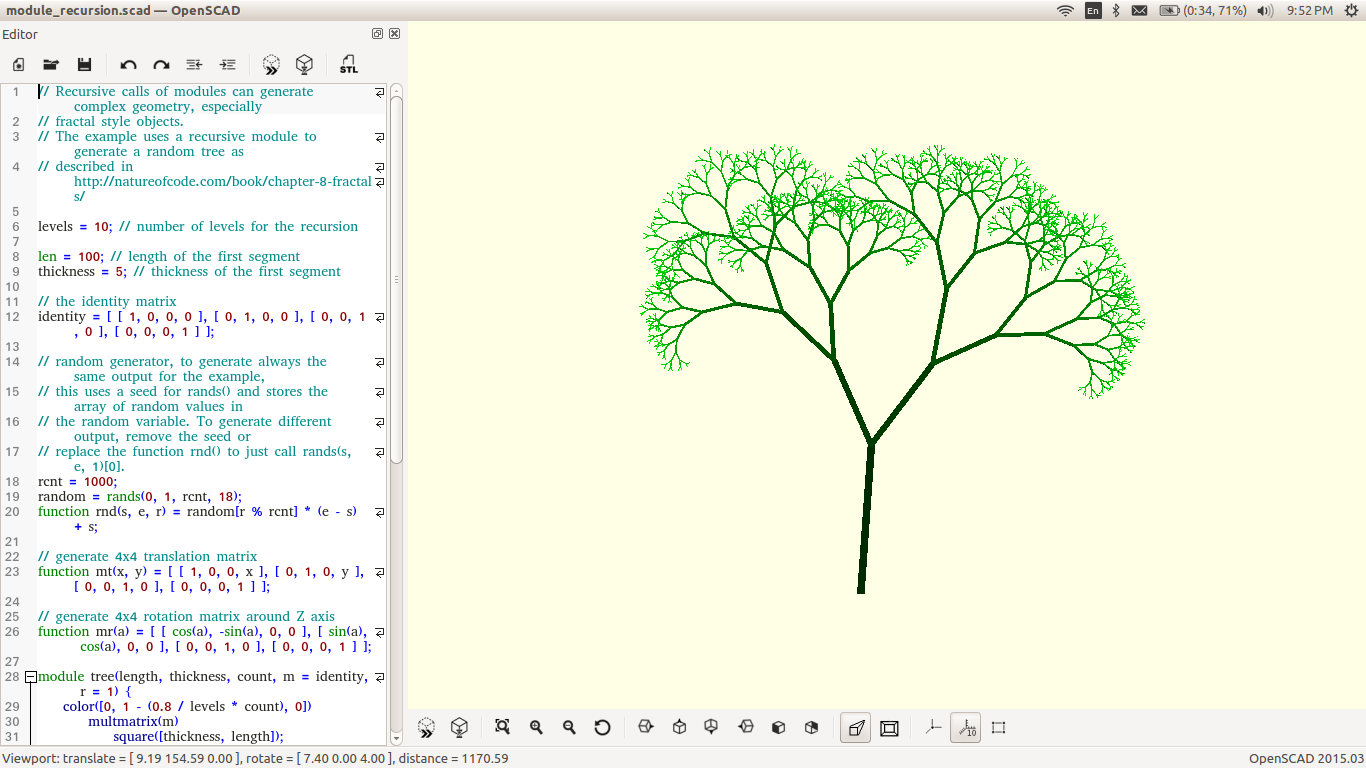
\includegraphics[scale=0.31]{images/output/2.png}
   	\caption{OpenSCAD without customizer}
   	\label{fig:Normal OpenSCAD}
\end{figure}
\begin{figure}[H] 
   	\centering 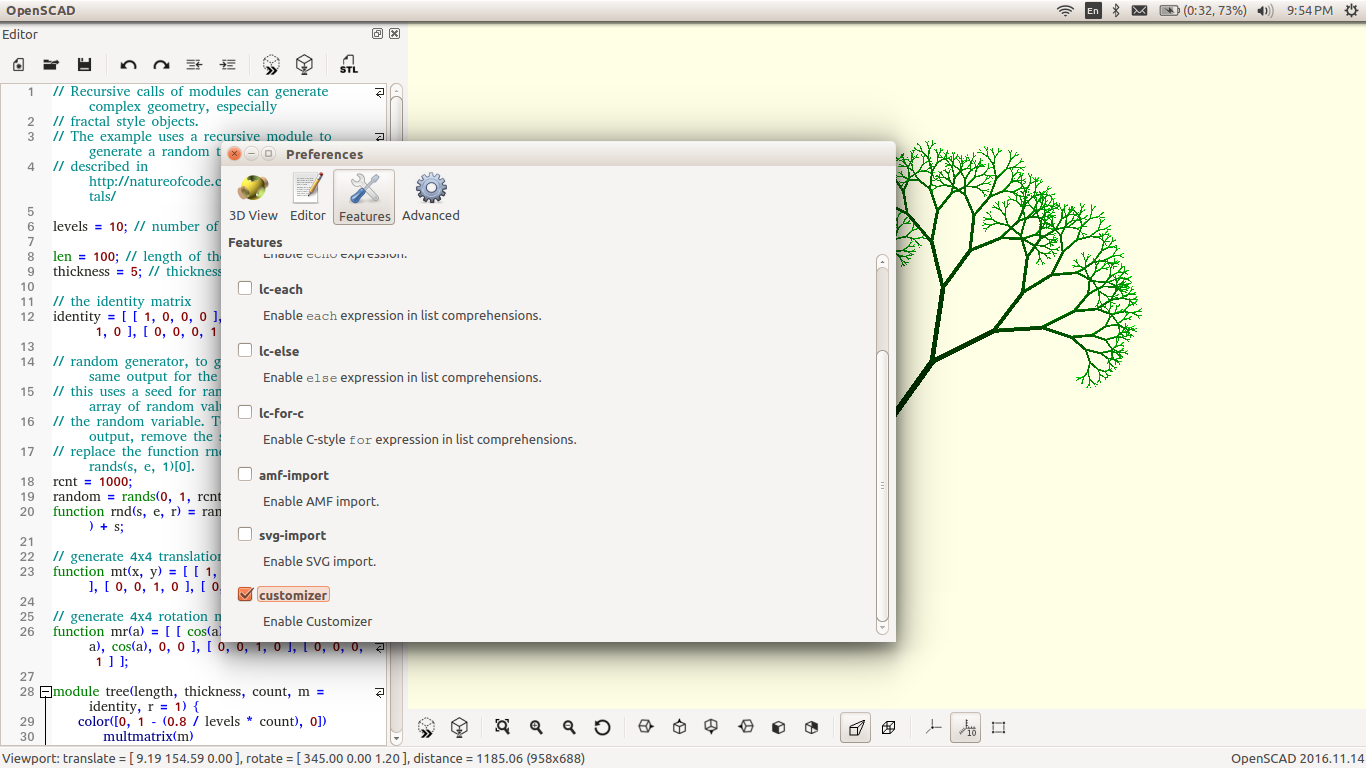
\includegraphics[scale=0.31]{images/output/3.png}
   	\caption{Preferences Widget to activate Customizer}
   	\label{fig:3}
\end{figure}
\begin{figure}[H] 
   	\centering 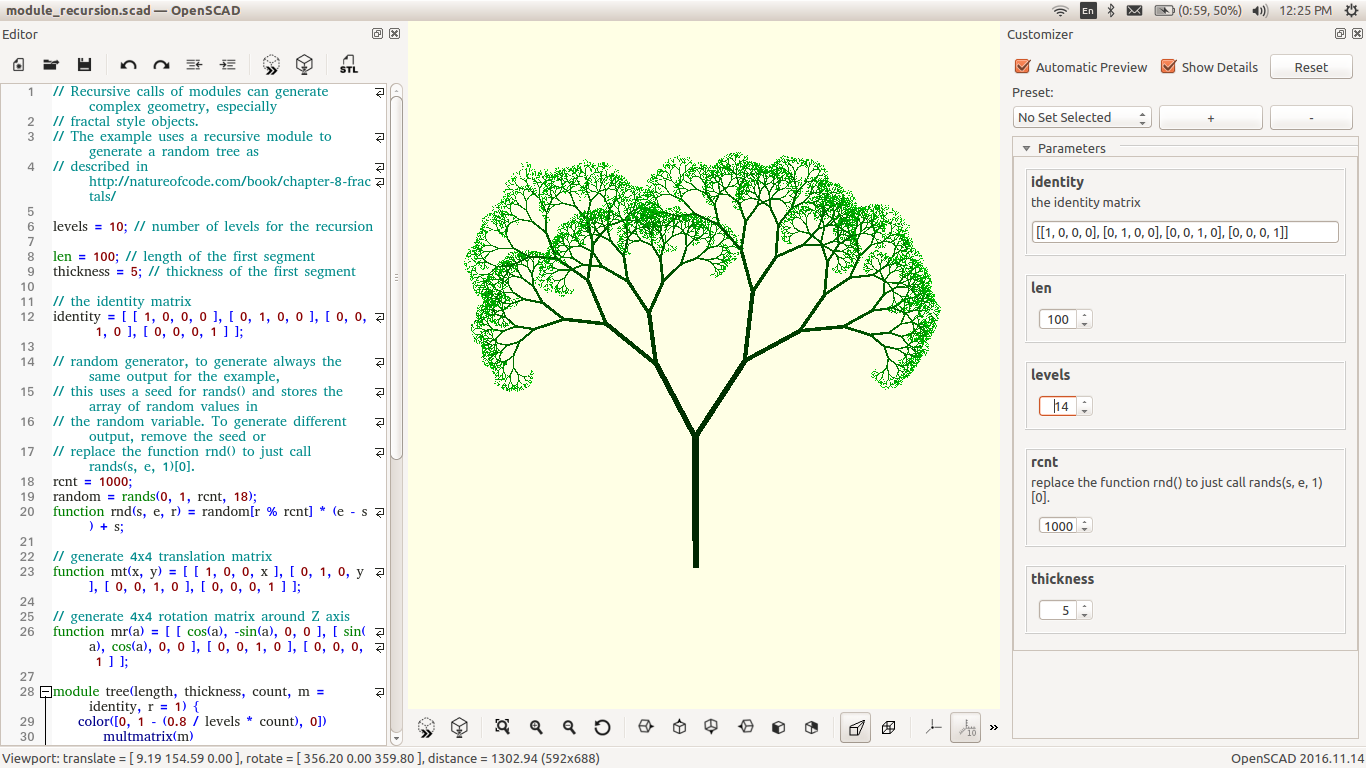
\includegraphics[scale=0.32]{images/output/5.png}
   	\caption{OpenSCAD with Customizer }
   	\label{fig:OpenSCAD with Customizer}
\end{figure}  

\subsection{Syntax support for generation of the customization form}

	\begin{lstlisting}[language=c++]
	// variable description
	variable name = defaultValue; // possible values
	\end{lstlisting}

Following is the syntax for how to define different types of widgets in the form

\begin{enumerate}
	\item \textbf{Drop down box}
	\begin{lstlisting}[language=c++]
	// combo box for nunber
	Numbers=2; // [0, 1, 2, 3]
	
	// combo box for string
	Strings="foo"; // [foo, bar, baz]
	
	//labeled combo box for numbers
	Labeled_values=10; // [10:L, 20:M, 30:L]
	
	//labeled combo box for string
	Labeled_value="S"; // [S:Small, M:Medium, L:Large]
	\end{lstlisting}
	\item \textbf{Slider} Only numbers are allowed in this one, specify any of the following:
	\begin{lstlisting}[language=c++]
	// slider widget for number
	slider =34; // [10:100]
	
	//step slider for number
	stepSlider=2; //[0:5:100]
	\end{lstlisting}
	\item \textbf{Checkbox}
	\begin{lstlisting}[language=c++]
	//description
	Variable = true;
	\end{lstlisting}
	\item \textbf{Spinbox}
	\begin{lstlisting}[language=c++]
	// spinbox with step size 1
	Spinbox= 5;
	\end{lstlisting}
	\item \textbf{Textbox}
	\begin{lstlisting}[language=c++]
	//Text box for vector with more than 4 elements
	Vector=[12,34,44,43,23,23];
	
	// Text box for string
	String="hello";
	
	\end{lstlisting}
	\item \textbf{Special vector}
	\begin{lstlisting}[language=c++]
	
	//Text box for vector with less than or equal to 4 elements
	Vector2=[12,34,45,23];
	\end{lstlisting}

\end{enumerate}

\subsection{Creating Tabs}
Parameters can be grouped into \textbf{tabs}. This feature will allow us to separate similar and related parameters. The syntax for this is also mainly similar to that of Thingiverse syntax for creating the tabs. To create a tab, use a multi-line block comment like this:

\textbf{/* [Tab Name] */}

The following tab names are reserved for special functionality:
\begin{description}
\item [Global] Parameters in the global tab will always be shown on every tab no matter which tab is selected. Note: there will be no tab for “Global” params, they will just always be shown in all the tabs.

\item [Hidden] Parameters in the hidden tab will never be displayed. Not even the tab will be shown. Even though the variables who have not been parameterized using the thingiverse or native syntax will not be displayed in openscad parameter widget but we have implemented this to make our comment like syntax similar as that of thinigverse.
\end{description}

Also the parameters who are under no tab will be diplayed under TAB named “parameters”.
\begin{lstlisting}[language=c++]
	/* [Drop down box:] */
	// combo box for nunber
	Numbers=2; // [0, 1, 2, 3]
	
	// combo box for string
	Strings="foo"; // [foo, bar, baz]
	
	//labeled combo box for numbers
	Labeled_values=10; // [10:L, 20:M, 30:XL]
	
	//labeled combo box for string
	Labeled_value="S"; // [S:Small, M:Medium, L:Large]
	
	/*[ Slider ]*/
	// slider widget for number
	slider =34; // [10:100]
	
	//step slider for number
	stepSlider=2; //[0:5:100]
	
	/* [Checkbox] */
	
	//description
	Variable = true;
	
	/*[Spinbox] */
	
	// spinbox with step size 1
	Spinbox = 5; 
	
	/* [Textbox] */
	
	//Text box for vector with more than 4 elements
	Vector=[12,34,44,43,23,23];
	
	// Text box for string
	String="hello";
	
	/* [Special vector] */
	//Text box for vector with less than or equal to 4 elements
	Vector2=[12,34,45,23];
\end{lstlisting}

\begin{figure}[H] 
	\centering 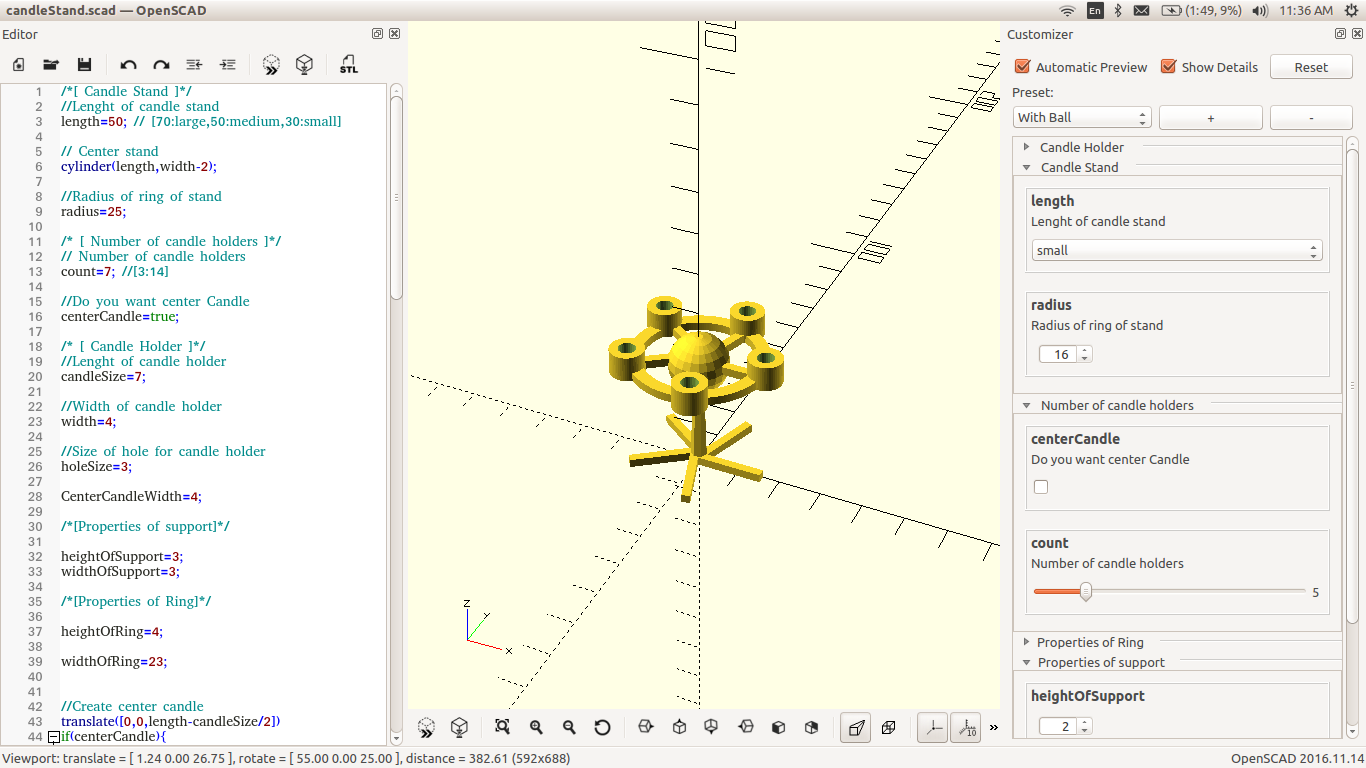
\includegraphics[scale=0.31]{images/output/6.png}
	\caption{First page of PDF generated by DoS}
	\label{fig:5}
\end{figure}

\subsection{ Saving Parameters value in JSON file}
This feature which is unique to openSCAD give user the ability to save the values of all parameters and also we can apply them through the cmd-line and get the output.

And JSON file is written in the following format:

\begin{lstlisting}[language=Java]
{
	"parameterSets":
	{
		    "fileFormatVersion": "1"
		"set-name ":
		{
			"parameter-name" :"value",
			"parameter-name" :"value"
		},
		"set-name ":{
			"parameter-name" :"value",
			"parameter-name" :"value"
		},
	},
	"fileFormatVersion": "1"
}
\end{lstlisting}

\textbf{Example:}
\begin{lstlisting}[language=Java]
{
	"parameterSets":
	{
		"FirstSet":
		{
			"Labled_values": "13",
			"Numbers": "18",
			"Spinbox": "35",
			"Vector": "[2,34,45,12,23,56]",
			"slider": "2",
			"stepSlider": "12",
			"string": "he"
		},
		"SeconSet":
		{
			"Labled_values": "10",
			"Numbers": "8",
			"Spinbox": "5",
			"Vector": "[12,34,45,12,23,56]",
			"slider": "12",
			"stepSlider": "2",
			"string": "hello"
		}
	},
	"fileFormatVersion": "1"
}
\end{lstlisting}

You can write the JSON file using the two methods:
\begin{itemize}
	\item Manually writting the JSON file
	\item Using the OpenSCAD's Customizer GUI
\end{itemize}

\subsection{Appling Parameters sets from JSON file}
To select the parameter set from the JSON file and apply them on model. We havae two options:

\begin{itemize}
	\item Cmdline
	\item GUI
\end{itemize}

\subsubsection{Cmdline}
\begin{lstlisting}[language=bash]
openscad --enable=customizer -o model-2.stl -p parameters.json -P model-2 model.scad
\end{lstlisting}

\begin{lstlisting}[language=bash]
openscad --enable=customizer -o <output-file> -p <parameteric-file> -P <NameOfSet> <input-file SCAD file >\end{lstlisting}

\begin{itemize}
	\item -p is used to give input JSON file in which parameters are saved.
	\item -P is used to give the name of the set of the parameters written in JSON file.
\end{itemize}

\begin{figure}[H] 
	\centering 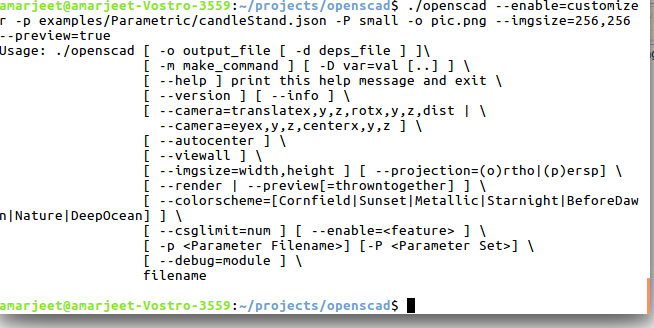
\includegraphics[scale=0.31]{images/output/8.png}
	\caption{Graph Generated in PDF}
	\label{fig:7}
\end{figure}

\subsubsection{GUI}

Through GUI you can easily apply and save Parameter in JSON file using Present section in Customizer explained below. 

In customizer, You will be able to see two checkbox’s which are
\begin{itemize}
\item [Automatic Preview] 
If checked preview of model will be automatically updated when you change any parameter in Customizer else you need to click preview button after you update parameter in customizer.
\item [Show Details] 
If checked the description for parameter will be shown above the input widget for the parameter else It will not be displayed but you still can view the description by hovering the cursor over the input widget.
\end{itemize}
Then comes \textbf{Reset} button which when clicked resets the values of all input widgets for the parameter to default provided in SCAD file.

Next come Preset section: It consist of three buttons
\begin{description}
	\item[combo Box] 
		It is used to select the set of parameters to be used
	\item[+ button]
	\begin{enumerate}
		\item It is used to update the set selected in combo Box. On clicking + button values of parameters in set are replaced by new values
		\item If we select “No set selected” in comboBox, then we can use + button to add new set of the parameters \ref{fig:Add new set}
	\end{enumerate}
	\begin{figure}[H] 
		\centering 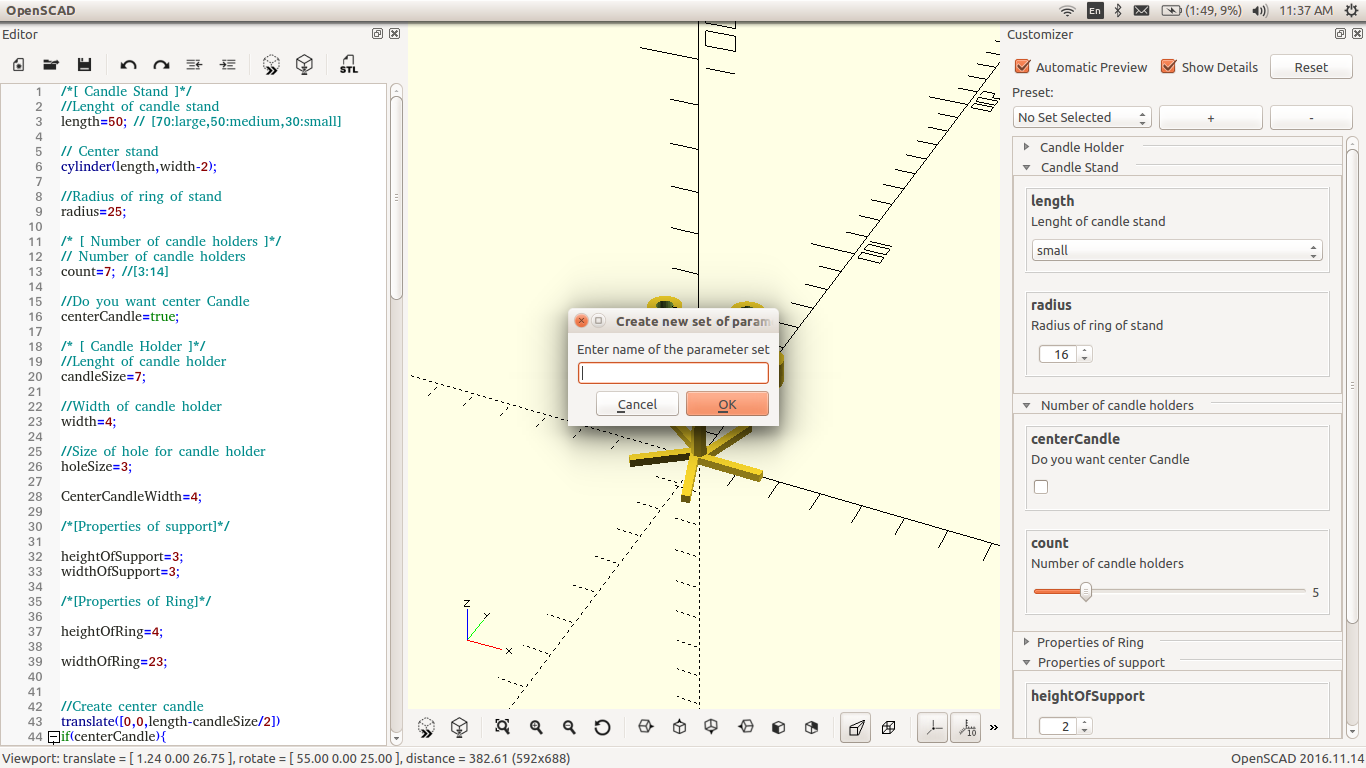
\includegraphics[scale=0.31]{images/output/7.png}
		\caption{Widget to add new set to JSON file}
		\label{fig:Add new set}
	\end{figure}

	\item [$-$ button] 
		It is used to delete the set selected in combo Box.
	and finally below Preset Section is the Place where you can play with the parameters.
\end{description}


You can also refer to  two examples that are Part of OpenSCAD to learn more
\begin{enumerate}
	\item Parametric/sign.scad
	\item Parametric/candlStand.scad
\end{enumerate}

After running a set of commands of \LaTeX and SageMath, it produces the
output in PDF form (with pdflatex) Figure \ref{fig:5}.

\begin{figure}[H] 
\centering 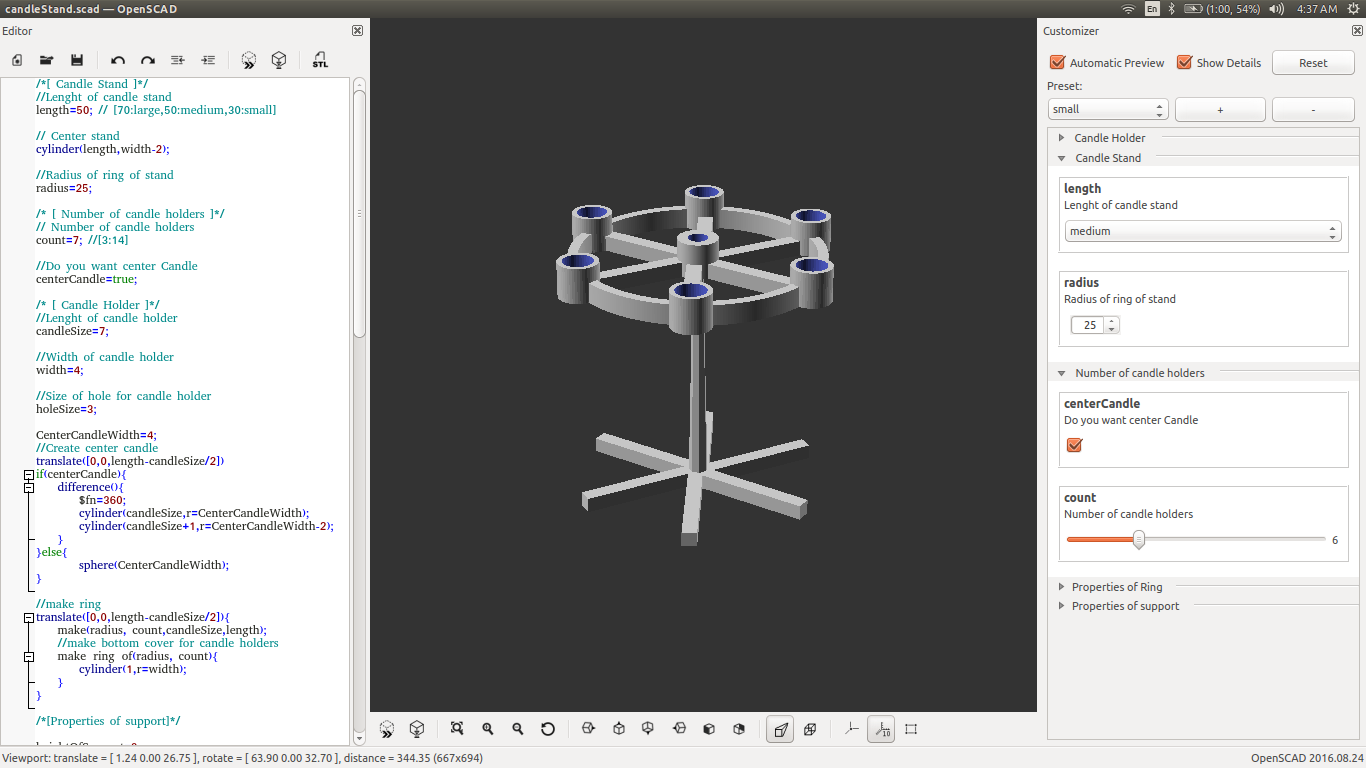
\includegraphics[scale=0.31]{images/output/9.png}
\caption{Final output in PDF}
\label{fig:8}
\end{figure}
